% Define document class. Options: article, report, book, ...
% \documentclass[twoside]{report} % use this if document is printed
\documentclass{report}  % use this if document only used as pdf

% Include preamble.tex
% Needed to add contents to toc without hyperlink
\let\origcontentsline\contentsline
\let\origaddtocontents\addtocontents

% Include packages
\usepackage[utf8]{inputenc}
% caption is used to jump to top of image, table and not to caption.
\usepackage{amsmath, amsfonts, amsthm, graphicx, tabularray, adjustbox, geometry, lipsum, caption, setspace, fancyvrb, fancyhdr, lastpage, etoolbox, xcolor, tikz, tcolorbox, siunitx, tocloft, hyperref, float, pdfpages}
\usepackage[Lenny]{fncychap} %Options: Sonny, Lenny, Glenn, Conny, Rejne, Bjarne, Bjornstrup
\usepackage[acronym]{glossaries-extra}
\usepackage[hyperref=true, backref=true, backend=biber, style=apa, sorting=nyt]{biblatex}

% Set page margins (package: geometry)
\newgeometry{
    top=3cm,
    bottom=2.5cm,
    outer=4cm,
    inner=4.5cm
}

% Set title of pdf and color of internal and external links (package: hyperref)
\hypersetup{
    linktoc=all,
    colorlinks=true,
    linkcolor=black,
    citecolor=black,
    urlcolor=blue,
    pdftitle={Bachelor Thesis}
}

% Needed so that hyperref also works in combination with \appendix
\renewcommand{\theHchapter}{\thepart.\thechapter}

% Set pagestyle of the first page of a new chapter to chapterstart (package: etoolbox)
\patchcmd{\chapter}{plain}{chapterstart}{}{}
% Declare chapterstart and plain pagestyle to have no line, no headers and no footers (package: fancyhdr)
\fancypagestyle{plain}{%
  \renewcommand{\headrulewidth}{0pt} % clear rules
  \fancyhf{} % Clear all header and footer fields.
}
\fancypagestyle{chapterstart}{%
  \renewcommand{\headrulewidth}{0pt} % clear rules
  \fancyhf{} % Clear all header and footer fields.
}

% Set default pagestyle to fancy and declare headers and footers. (package: fancyhdr)
\pagestyle{fancy}
\renewcommand{\chaptermark}[1]{\markboth{#1}{}}
\renewcommand{\sectionmark}[1]{\markright{#1}{}}
\cfoot{} % clear default page number in center
% Use the following for alternating headers if doucment is printed
%\fancyhead{} % clear all header fields
%\fancyhead[LO,RE]{\nouppercase\leftmark}
%\fancyhead[RO,LE]{\thepage}
% Use following for static headers if document only used as pdf
\lhead{\nouppercase\leftmark}
\rhead{\thepage}
%\rfoot{Page \thepage\ of \pageref{LastPage}}

% Format chapter title (package: fancychap)
\ChNameUpperCase
%\ChNumVar{\fontsize{40}{42}\usefont{OT1}{ptm}{m}{n}\selectfont}
\ChTitleVar{\huge\sc}

% Increase space between text by 50 % (package: setspace)
\onehalfspacing 

% Increase space between table rows by 0.3 em (package: tabularray)
\SetTblrInner{rowsep=0.3em}

% Remove indentation in list of figures and list of tables
\makeatletter
\renewcommand*\l@figure{\@dottedtocline{1}{0em}{2.3em}} % Default: 1.5em/2.3em
\let\l@table\l@figure
\makeatother

% Define acronym style and create glossary (package: glossaries-extra)
\setabbreviationstyle[acronym]{long-short}
\makeglossaries

% Add bib resource and configure blibliography (package: biblatex)
\addbibresource{ref.bib}
\DefineBibliographyStrings{english}{%
    backrefpage  = {\lowercase{s}ee p.}, % for single page number
    backrefpages = {\lowercase{s}ee pp.} % for multiple page numbers
}
\newcommand{\apacite}[1]{(\cite{#1})}
\DeclareBibliographyAlias{artwork}{online} % use online entry type for artwork entries

% Add commands for adding list of equations (package: tocloft)
\newcommand{\cftloetitlefont}{} % new command which allows to format title font of list of equations
\newcommand{\listequationsnamedefaultformat}{List of Equations}
\newcommand{\listequationsname}{\cftloetitlefont{\listequationsnamedefaultformat}}
\newlistof{myequations}{equ}{\listequationsname}
\newcommand{\myequations}[1]{\addcontentsline{equ}{myequations}{\protect\numberline{\theequation}#1}\par}

% Reformat headings of listings (package: tocloft)
\renewcommand\cfttoctitlefont{\huge\sc} % toc
\renewcommand\cftloftitlefont{\huge\sc} % list of figures
\renewcommand\cftlottitlefont{\huge\sc} % list of tables
\renewcommand\cftloetitlefont{\huge\sc} % list of equations

% Add auto indentation to captions (package: caption)
\captionsetup{format=hang}

% Include acronyms and glossary declarations
\newacronym{sota}{SotA}{state-of-the-art}
\newacronym{hslu}{HSLU}{Lucerne University of Applied Sciences and Arts}
\newacronym{cnn}{CNN}{Convolutional Neural Network}
%\newacronym{}{}{}
\newglossaryentry{latex}
{
    name=latex,
    description={Is a markup language specially suited 
    for scientific documents}
}

\newglossaryentry{maths}
{
    name=mathematics,
    description={Mathematics is what mathematicians do}
}

% Start of document content
\pagenumbering{roman}
\begin{document}
\begin{sloppypar}

\thispagestyle{empty}
\begin{figure}[ht]
    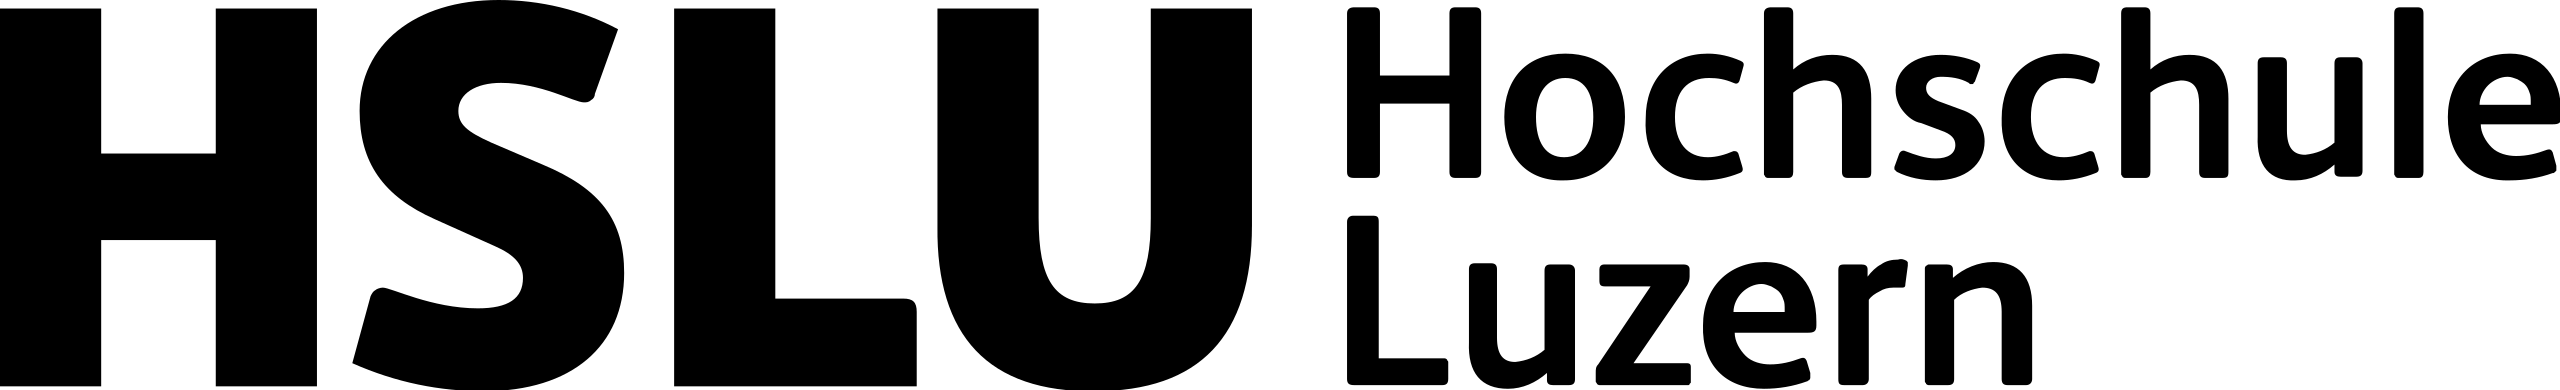
\includegraphics[width=20em,height=\textheight,keepaspectratio]{images/hslu_2022_logo.png}
\end{figure}
\vspace*{9em}

\noindent\begin{center}
\huge{\textbf{Machine Learning for the Prediction of Refractive Surprise after Cataract Surgery}}\\
\vspace*{3em}

\Large{Bachelor Thesis}\\
\Large{B.Sc. in Computer Science}\\
\vspace*{4em}

\Large{by}\\
\Large{\textbf{Your Name}}\\
\Large{03\textsuperscript{th} of January 2023}\\
\vspace*{\fill}

\large{Advisors:\\Dr. John Doe, Dr. sc. ETH Max Mustermann}
\end{center}
\thispagestyle{empty}
\vspace*{\fill}
\begin{center}
    \copyright\ 2023\\
    Your Name\\
    ALL RIGHTS RESERVED
\end{center}
\chapter*{Declaration}
\chapter*{Abstract}

% Add empty page for double sided print
\newpage 
\thispagestyle{empty}
\ % The empty page
\newpage
\chapter*{Acknowledgements}

\chapter*{Demo}
\section*{Cite}
Test cite \apacite{yamauchi_use_2021}.

\section*{Hyperref}
Test Href \href{http://google.ch}{Google}. You can also jump to a chapter or section (see \ref{ch:introduction}). We can also jump to the appendix (see \ref{app:original_project_description}).

\section*{fancyvbr}

\begin{Verbatim}[numbers=left, frame=single]
client = RestClient("localhost:80", "application/json")
students = client.Get("/api/students")
\end{Verbatim}

\section*{color}
Make {\color{red} this} red.

\section*{tcolorbox}
\begin{tcolorbox}
This is a tcolorbox.
\end{tcolorbox}

\section*{Glossary}
The \gls{latex} typesetting markup language is specially suitable 
for documents that include \gls{maths}. 

\section*{Acronym}
This is a \gls{cnn} and the second \gls{cnn}.

\section*{SI units}
\[5 kg m /s^2\]

\[5\ \mathrm{kg}\ \mathrm{m}/\mathrm{s}^2\]

\[5\ \si{kg.m/s^2}\]

\section*{Tables}
\subsection*{Simple Table}
In this thesis you should always use a forward reference for your tables \ref{tab:demo}.
\begin{table}[ht]
\centering
\begin{adjustbox}{max width=\textwidth}
\begin{tblr}{ l|l|l } 
 metric & average & other \\ 
 \hline
 accuracy & 90 \% & 65 \% \\ 
 precision & 81 \% & 70 \% \\
 f1 & 87 \% & 63 \% \\ 
\end{tblr}
\end{adjustbox}
\caption{This is a demo caption for a simple table.}
\label{tab:demo}
\end{table}

The following table \ref{tab:reference_label_prefix} shows which prefix to use for different types of labels.
\begin{table}[ht]
\centering
\begin{adjustbox}{max width=\textwidth}
\begin{tblr}{ l|l l l l l l l }
 Name & Chapter & Section & Subsection & Equation & Figure & Table & Appendix \\
 \hline
 Abbrev. & ch: & sec: & subsec: & eq: & fig: & tab: & app: \\
\end{tblr}
\end{adjustbox}
\caption{Add some letters to the label to recognize what you are referencing.}
\label{tab:reference_label_prefix}
\end{table}


\section*{Figures}
In this thesis you should always use a forward reference for your figures \ref{fig:demo}.
\begin{figure}[ht]
    \centering
    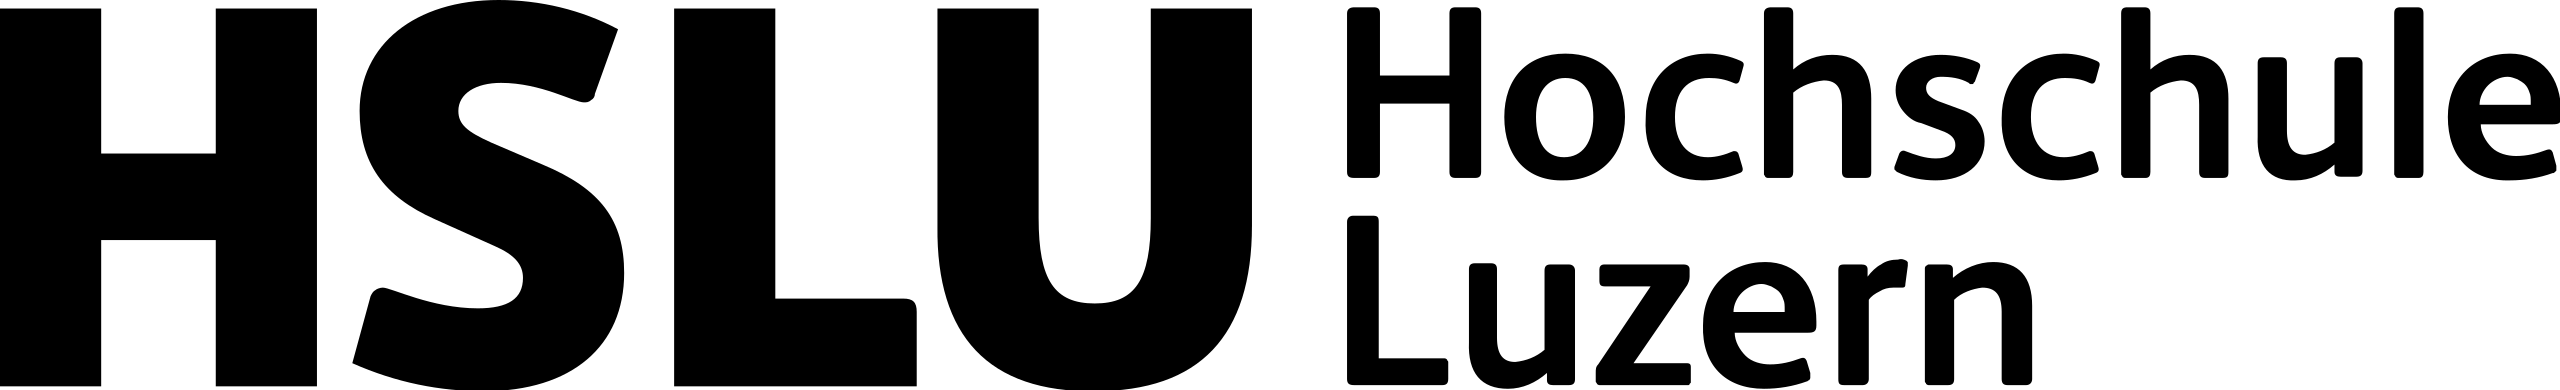
\includegraphics[width=\textwidth,height=\textheight,keepaspectratio]{images/hslu_2022_logo.png}
    \caption{This is a demo caption for a figure.}
    \label{fig:demo}
\end{figure}

\tableofcontents

\pagenumbering{arabic}
\chapter{Introduction}\label{ch:introduction}
\lipsum[1-10]
\chapter{State of Research}\label{ch:state_of_research}

\chapter{Concept}\label{ch:concept}
\chapter{Methodology}\label{ch:methodology}
\chapter{Realization}\label{ch:realization}
\chapter{Evaluation}\label{ch:evaluation}
\chapter{Conclusion}\label{ch:conclusion}

\appendix
\part*{Appendix}
\origaddtocontents{toc}{\protect\origcontentsline{part}{Appendix}{}\%}
\chapter{Original Project Description}\label{app:original_project_description}
Following the original project description in German as created in JointCreate \apacite{jointcreate_project}.

\section{Ausgangslage und Problemstellung}
Die Katarakt oder Grauer Star ist eine Trübung der Augenlinse, die zu einem langsam fortschreitenden Verlust der Sehschärfe führt. Die Katarakt tritt bei ca. jeder sechsten Person über 40 Jahren auf. Bei der Kataraktoperation wird die trübe Linse durch ein künstliches Implantat ersetzt. Die Kataraktoperation ist die heute weltweit am häufigsten durchgeführte Operation. Alleine in Deutschland werden rund 950.000 Eingriffe pro Jahr durchgeführt. Die exzellente Erfolgsquote und Zufriedenheit der Patienten im Allgemeinen täuscht darüber hinweg, dass bei wenigen Prozent der Patienten refraktive Überraschungen oder Komplikationen auftreten, so dass hier ggf. Folgeeingriffe nötig sind bis hin zur Explantation / zum Ersatz der Linse. Oft werden dabei Premiumlinsen mit Zusatzfunktionen gegen deutlich besser tolerierte Standardlinsen ausgetauscht.

Viele der refraktiven Überraschungen sollten vermeidbar sein, wenn entsprechende Screeningverfahren vorhanden wären welche die vor dem Eingriff erhobenen biometrischen Daten sowie patientencharakteristische Größen abgleichen und dem Operateur eine Warnung an die Hand geben, z.B. von Premiumlinsen (multifokale oder torische Linsen) abzusehen.

\section{Datenmaterial}
Zur Verfügung stehen einige Tausend vor einer Kataraktoperation erhobene biometrische Messungen (mit dem IOLMaster700 der Firma Carl-Zeiss-Meditec, vollständige Datensätze), patientencharakteristische Daten wie das Alter und Geschlecht, der Brechwert und Typ der implantierten Linse, sowie das refraktive Ergebnis nach der Operation. Der Brechwert der zu implantierenden Linse bzw. die zu erwartenden Refraktion nach dem Eingriff können mit den biometrischen Größen abgeschätzt werden, so dass die Abweichung der tatsächlich gemessenen Refraktion von der vorhergesagten Refraktion als "Refraktionsüberraschung" definiert ist.

\section{Ziel der Arbeit und erwartete Resultate}
In dieser Arbeit soll ein Machine Learning Verfahren entwickelt werden, mit dem die Refraktionsüberraschung vorhergesagt werden kann. Dabei ist sowohl eine Vorhersage in Form einer Klassifizierung (deutliche/mittlere/geringe Abweichung in Richtung Myopie/Hyperopie) oder auch kontinuierliche Vorhersage (Regression) möglich.

Abgegeben werden soll ein Bericht mit State-of-the-Art, Konzept, Ansätzen, der/den entwickelten Methoden und einer robusten Evaluation, sowie lauffähiger, kommentierter Programmcode.

\section{Gewünschte Methoden, Vorgehen}
Bei diesem Projekt handelt es sich um explorative Forschung, das in einem iterativen, inkrementellen Ansatz umgesetzt werden soll. Die/der Student:in soll den aktuellen Stand des Projektes und die nächsten Schritte in regelmässigen Absprachen mit dem Betreuer besprechen, um Feedback zu sammeln und sich zu verbessern. Dabei gilt es, den Fokus auf der Entwicklung eines Vorhersage-Algorithmus zu halten und diesen im Sinne einer Machbarkeitsstudie zu entwickeln und zu testen.

Darüber hinaus müssen Risiken so früh wie möglich gesammelt, verfolgt und gemindert werden, um zu überprüfen, ob einige Risiken ein Hindernis für das Projekt darstellen.

\section{Kreativität, Varianten, Innovation}
Das Projektziel ist bewusst offen formuliert und lässt viel Raum für eigene Kreativität.

Die Auswahl und Umsetzung des geeigneten Projektvorgehens ist Teil der Projektaufgabe und liegt grundsätzlich in der Verantwortung der/s Student:in. In regelmäßigen Treffen mit dem Betreuer werden der aktuelle Stand und die nächsten Schritte besprochen.

Der Betreuer soll regelmässig bis einen Tag vor dem geplanten Treffen schriftlich (max. 1 Seite) über den aktuellen Stand informiert werden:

\begin{itemize}
  \item Welche Arbeiten wurden im letzten Berichtszeitraum durchgeführt, welche Arbeiten sind für die nächste Periode geplant
  \item Stand der Arbeiten (Soll-Ist-Vergleich mit Planung), ggf. Begründung von Abweichungen
  \item Top-3-Risiken inklusive geplanter Maßnahmen
\end{itemize}

Die Architektur soll so einfach wie möglich gehalten werden. Bezüglich der Programmiersprache ist der/die Student:in frei; es sollen jedoch wenn möglich und sinnvoll vorhandene Open-Source-Bibliotheken (wie sklearn, pytorch, …) wiederverwendet werden, um das Ziel effizient zu erreichen.
\chapter{Minutes}\label{app:minutes}
\chapter{Milestones}\label{app:milestones}
\chapter{Risks}\label{app:risks}



\part*{Listings}
\origaddtocontents{toc}{\protect\origcontentsline{part}{Listings}{}\%}
\cleardoublepage
\phantomsection
\addcontentsline{toc}{chapter}{\listfigurename}
\listoffigures

\cleardoublepage
\phantomsection
\addcontentsline{toc}{chapter}{\listtablename}
\listoftables

\cleardoublepage
\phantomsection
\addcontentsline{toc}{chapter}{\listequationsnamedefaultformat}
\listofmyequations

\printglossary[type=\acronymtype]
\printglossary

\cleardoublepage
\phantomsection
\printbibliography[heading=bibintoc, title={Bibliography}]

\end{sloppypar}
\end{document}